% ==============================================================================
% LAB 119
% UNDERSÖKNING AV RC-KRETS
% ------------------------
% Last updated <2015-03-29>
%
% Author:
% Jonas Sjöberg     <tel12jsg@student.hig.se>
% Oscar Wallberg    <tco13owg@student.hig.se>
%
% License:
% Creative Commons Attribution-NonCommercial-ShareAlike 4.0 International
% See LICENSE.md for full licensing information.
% ==============================================================================

% ==============================================================================
% INCLUDES AND CONFIGURATION
% ==============================================================================
\documentclass[11pt,a4paper]{article}
\usepackage[utf8]{inputenc}
\usepackage[swedish]{babel} % För svensk innehållsförteckning
\usepackage{siunitx} % (För dokumentation, kör i terminalen; texdoc siunitx)
\usepackage{amssymb}
\usepackage{amsmath}
\usepackage{amsfonts}
\usepackage{graphicx}
\usepackage{booktabs}
\usepackage{longtable} % Tables span across pages
\usepackage{microtype}
\usepackage{gensymb}
%\usepackage{tabto}
\usepackage{units}

\setlength\parindent{0pt} % Removes all indentation from paragraphs

% ==============================================================================
% DOCUMENT METADATA
% ==============================================================================
\title{EE466 \\ Lab 119 \\ Undersökning av RC-krets}

\author{\\
  Jonas Sjöberg\\
  Högskolan i Gävle,\\
  Elektronikingenjörsprogrammet,\\
  \texttt{tel12jsg@student.hig.se}\\
  \\
  Oscar Wallberg\\
  Högskolan i Gävle,\\
  Dataingenjörsprogrammet,\\
  \texttt{tco13owg@student.hig.se}\\}

\date{}
% ==============================================================================
\begin{document}
% ==============================================================================
\maketitle

\begin{center}
    \begin{tabular}{l r}
        Labb utförd: & TODO: Labben utförd datum \\
        Instruktör: & Efrain Zenteno
    \end{tabular}
\end{center}

% ==============================================================================
% ABSTRACT
% ==============================================================================
\begin{abstract}
    Syftet med laborationen är att analysera funktionen hos en RC krets.
    Laborationen innefattar överföringsfunktionen för en RC-krets, i både tids-
    och frekvensdomänen. Stegsvaret för en första ordningens krets. Bode-diagram.
    Begreppen brytfrekvens, frekvens- och faskaraktäristik.
\end{abstract}

\newpage

{
    %\hypersetup{linkcolor=black}
    \setcounter{tocdepth}{3}
    \tableofcontents
}

\newpage

% ==============================================================================
% SECTION: INTRODUKTION
% ==============================================================================
\section{Introduktion}\label{setup}
% ==============================================================================
I denna labb skall vi studera en passiv krets uppbyggd av ett motstånd och en
kondensator. Om en sådan krets matas med en sinusformad insignal kommer den att
släppa igenom vissa frekvenser medan andra frekvenser dämpas. Ett sådant
frekvensberoende nät kallas därför ofta för filter. Om kretsen innehåller
endast en reaktiv (dvs energilagrande) komponent (spole eller kondensator)
kallar vi kretsen för ett första ordningens filter. Namnet kommer sig av att
kretsen kan beskrivas med en första ordningens differentialekvation.
Vi skall analysera kretsen både i frekvensplanet genom att mäta upp ett
Bode-diagram och i tidsplanet genom att mäta upp kretsens stegsvar.


% ==============================================================================
% SECTION: 1 UPPMÄTNING AV BODE-DIAGRAM 
% ==============================================================================
\section{Uppmätning av Bode-diagram}\label{}
% ==============================================================================

\subsection{Experimentuppställning}\label{}
% ------------------------------------------------------------------------------
En så kallad experimentplatta eller "breadboard" används för att konstruera
kretsen som illustreras i Figur \ref{fig:1-freqdom_schem}.
\par För att generera en sinusformad signal används signalgeneratorn HP33120A,
vars utgång kopplas genom en BNC-förgrening till oscilloskopet Agilent 54621A
och genom en BNC- banankontaktadapter, med "banankablar" till
breadboardplattans skruvterminaler.
\par Oscilloskopet visar signalen från kretsens ingång, dvs signalgeneratorns
utgångs, på kanal ett. Kanal två kopplas till kretsens utgång, Punkt A i
\ref{fig:1-freqdom_schem} med en oscilloskop-prob. Proben ställs till att dämpa
med en faktor av 10:1 och den vertikala skalan justeras en dekad nedåt, så att
båda kanalerna visas med samma skalfaktor.


\begin{figure}
    \centering
    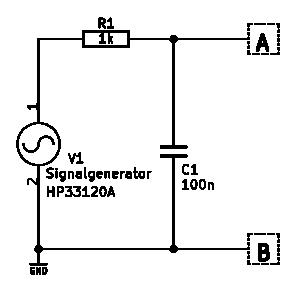
\includegraphics[width=0.6\linewidth]{img/1-freqdom_schem}
    \caption[Schematisk ritning av labbkoppling, första ordningens RC-filter.]
    {Schematisk ritning av labbkoppling, första ordningens RC-filter.}
    \label{fig:1-freqdom_schem}
\end{figure}


\subsection{Mätresultat}\label{}
% ------------------------------------------------------------------------------
% TODO:

\subsection{Kommentar}\label{}
% ------------------------------------------------------------------------------
% TODO:


% ==============================================================================
% SECTION: 2 UPPMÄTNING AV STEGSVARET 
% ==============================================================================
\section{Uppmätning av stegsvaret}\label{}
% ==============================================================================
% TODO: 

\subsection{Mätresultat}\label{}
% ------------------------------------------------------------------------------
% TODO:

\subsection{Kommentar}\label{}
% ------------------------------------------------------------------------------
% TODO:


% ==============================================================================
% SECTION: 3 INVERKAN AV KÄLLIMPEDANS OCH BELASTNINGSIMPEDANS 
% ==============================================================================
\section{Inverkan av källimpedans och belastningsimpedans}\label{}
% ==============================================================================
% TODO: 

\subsection{Mätresultat}\label{}
% ------------------------------------------------------------------------------
% TODO:

\subsection{Kommentar}\label{}
% ------------------------------------------------------------------------------
% TODO:


% ==============================================================================
% SECTION: RESULTAT
% ==============================================================================
\section{Resultat}\label{setup}
% ==============================================================================
Sammanfattningsvis kan sägas att laborationen innehåller en mängd koncept som
är mycket viktiga att få en grundlig förståelse för. Vi har inte stött på några
direkta problem.

\newpage

% ==============================================================================
% SECTION: REFERENSER
% ==============================================================================
\section{Referenser}\label{refs}
% ==============================================================================
%TODO: Referenser.

%\subsection{www}\label{interwebs}
% ------------------------------------------------------------------------------

%\subsection{Trycksaker}\label{literature} %???
% ------------------------------------------------------------------------------

%\subsection{Källkod}\label{sourcefiles}
% ------------------------------------------------------------------------------

% ==============================================================================
\end{document}
% ==============================================================================
